\section{Данные}

\subsection{VisDrone}

VisDrone -- набор из 288 видео, сформированный из 261,908 кадров и 10,209 статических изображений, полученных с помощью различных камер с беспилотных летательных аппаратов в городах Китая при разных погодных условиях и варьирующейся освещенности, с различным количеством объектов и их плотностью в кадре, с разных ракурсов и позиций в воздушном пространстве, как показано на Рис. \ref{img:3-1}.

\vspace{0.5cm}

\begin{figure}[ht]
    \centering
    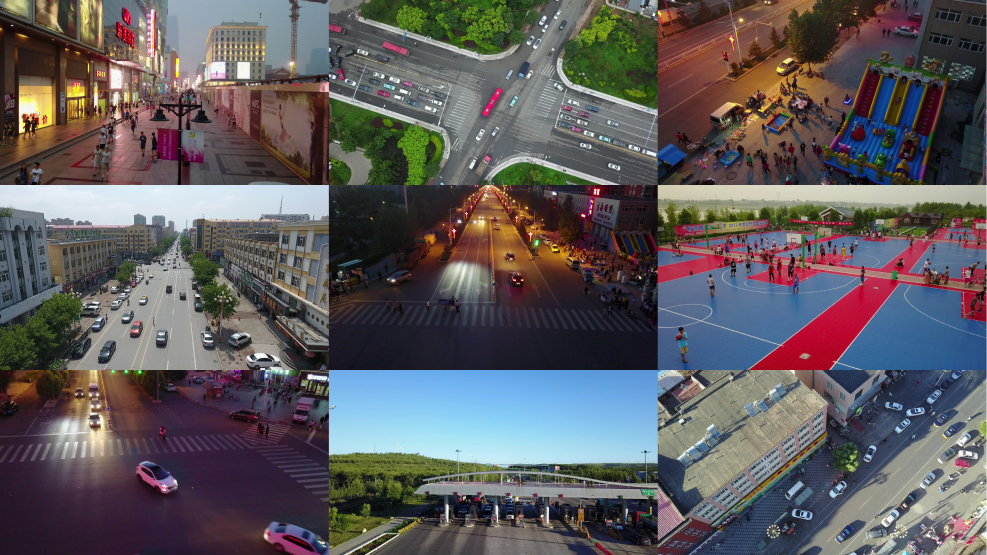
\includegraphics[width=0.85\textwidth]{3-1}
    \caption{Пример выборки кадров из VisDrone}
    \label{img:3-1}
\end{figure}

Датасет был создан командой AISKYEYE из лаборатории машинного обучения и сбора данных Тяньцзиньского университета в Китае с целью формирования базы для проведения оценки моделей и исследования алгоритмов визуального анализа, связанных с беспилотными летательными аппаратами. Все полученные материалы были вручную аннотированы при помощи 2.6 миллиона ограничивающих рамок, кадры с примерами которых представлены на Рис. \ref{img:3-2}.

\begin{figure}[ht]
    \centering
    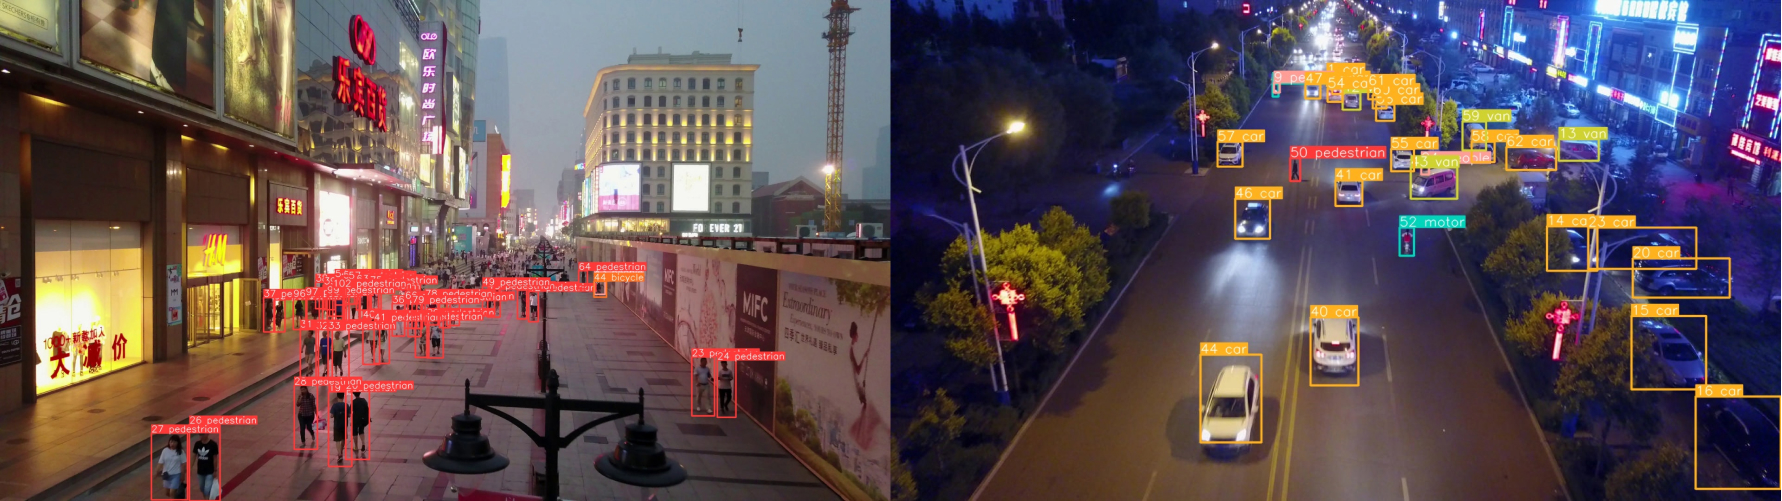
\includegraphics[width=0.85\textwidth]{3-2}
    \caption{Пример аннотированных кадров VisDrone}
    \label{img:3-2}
\end{figure}

Весь датасет подразделяется на 5 задач: детектирование объектов на изображениях, детектирование объектов на видео, трекинг одного объекта, трекинг множества объектов и подсчет количества людей в толпе. В датасете представлено 10 классов: pedestrian, person, car, van, bus, truck, motor, bicycle, awning-tricycle и tricycle.
Используемая в данной работе часть датасета -- VisDrone-MOT2019 -- состоит из 79 видеорядов из 33,366 кадров суммарно, из которых train -- 56 видеорядов из 24,198 кадров, val -- 7 видеорядов из 2,846 кадров, test -- 16 видеорядов из 6,322 кадров.

Следует заметить, что в датасете присутствует значительно выраженная несбалансированность классов, создающая видимые затруднения в классификации объектов, что наглядно показано на Рис. \ref{img:3-3}. Наиболее представленным является класс car, объем которого почти в 2.5 раза превышает второй по распространенности класс pedestrian и в 50 раз класс bus.

\begin{figure}[ht]
    \centering
    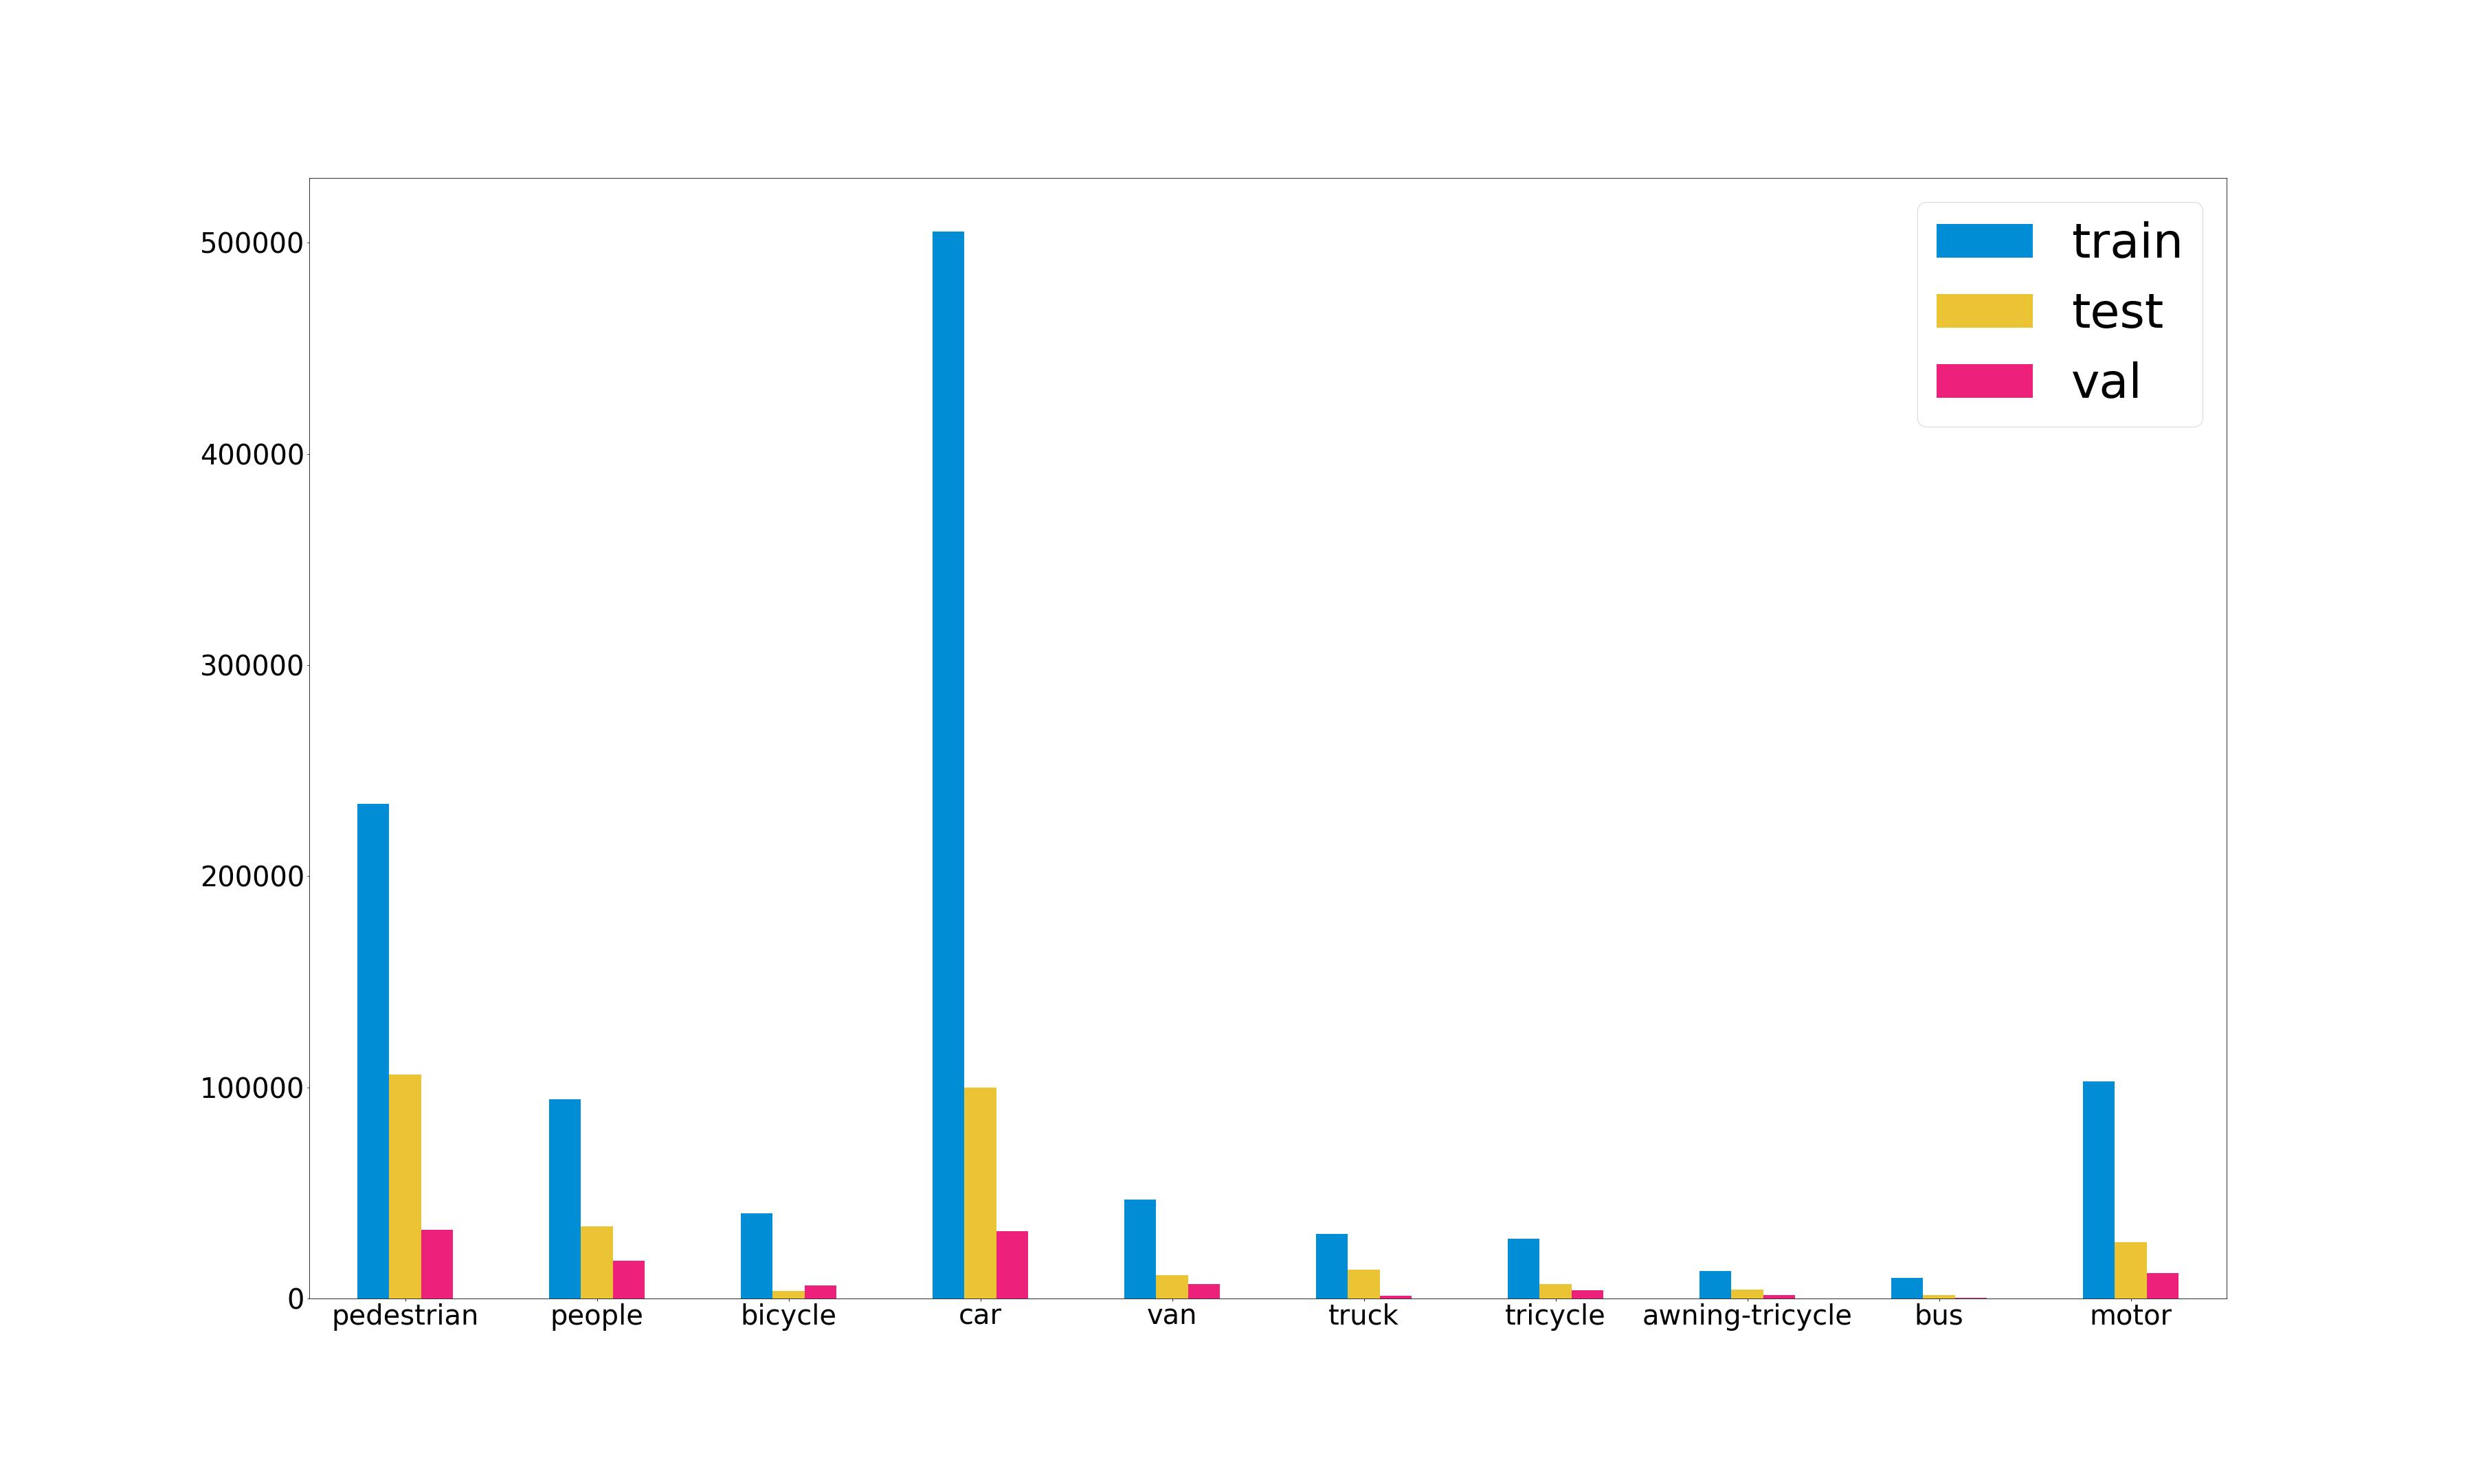
\includegraphics[width=0.85\textwidth]{3-3}
    \caption{Распределение объектов по классам в VisDrone-MOT2019}
    \label{img:3-3}
\end{figure}
